\section{Вычислительные эксперименты}
    В качестве функции тока возьмём:
    \[
        \psi(x, y) = \sin (2 \pi x) \sin(\pi y),
    \]

    откуда получаем:
    \[
        \left\{
            \begin{split}
                & u(x, y) = -\pi \sin (2 \pi x) \cos(\pi y), \\
                & v(x, y) = 2\pi \cos (2 \pi x) \sin(\pi y).
            \end{split}
        \right.
    \]

    \begin{figure}[H]
        \centering
        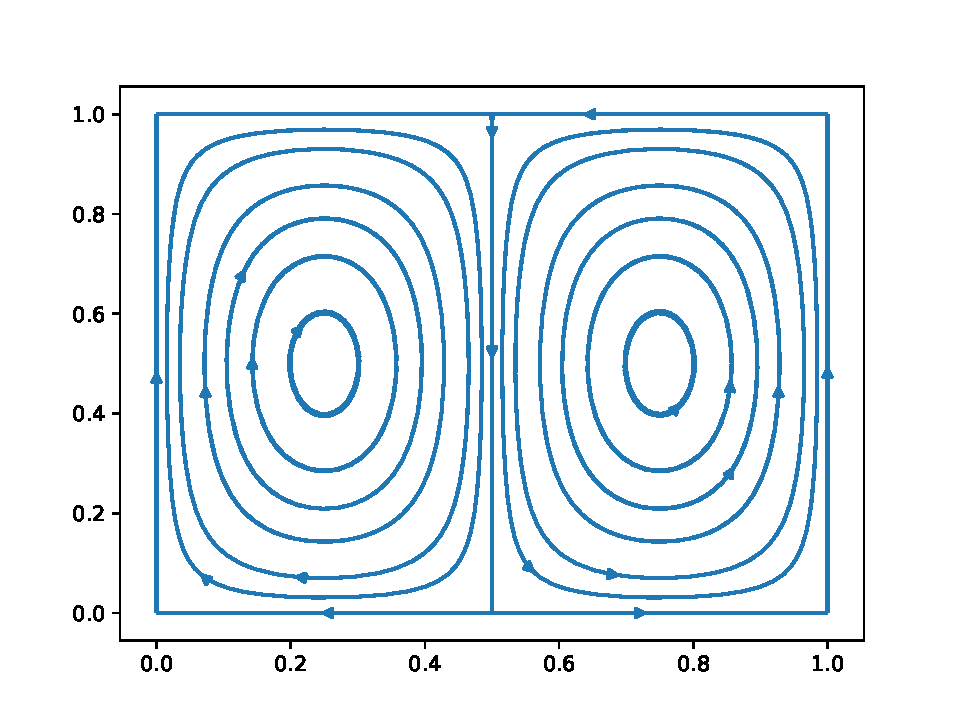
\includegraphics[width=12cm]{pictures/streamplot.pdf}
        \caption{Фазовые кривые функции тока \( \psi(x, y) \).}
    \end{figure}

    \[
        C_0(x, y) = \arctan \left( \frac{y - 0.5}{0.1} \right)
    \]

    \subsection{Алгоритм}
        Для реализации моделей сделаем замену переменных \( u(t) = \dot{x}(t), \quad v(t) = \dot{y}(t) \), и получим систему дифференциальных уравнений первого порядка:
        \[
            \left\{\begin{split}
                & \dot{x} = u, & \dot{y} = v, \\
                & \dot{u} = 2 \Omega v, & \dot{v} = -2 \Omega u, \\
                & x(0) = x_0, & y(0) = y_0, \\
                & u(0) = x_1, & v(0) = y_1.
            \end{split}\right.
        \]

        Для компьютерного вычисления будем использовать метод Рунге-Кутты, с помощью которого получим численное решение системы дифференциальных уравнений с заданными параметрами. После чего построим их решения и фазовые плоскости.

        По полученному закону сохранения энергии можем вывести соотношение: \( u^2 + v^2 - x_1^2 - y_1^2 = 0 \). Также проверим его выполнение для численного решения.



    \subsection{Программа}
        Для расчётов и визуализации был использован язык Python с библиотеками numpy и matplotlib.

    \subsection{Результаты}

    \begin{figure}[H]
        \centering
        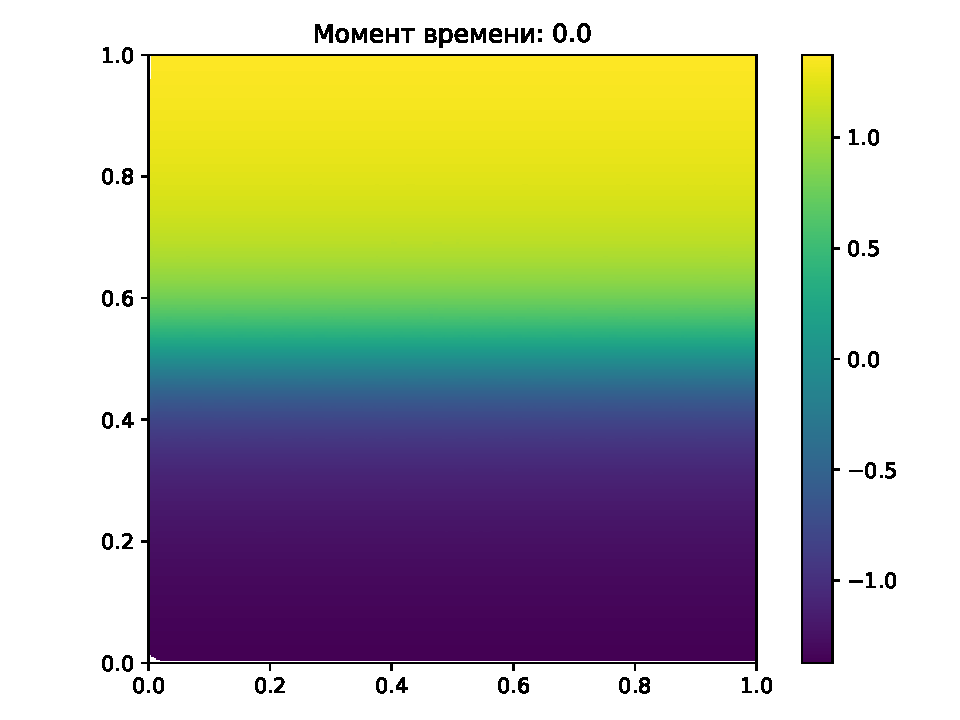
\includegraphics[width=8cm]{pictures/p0.pdf}
        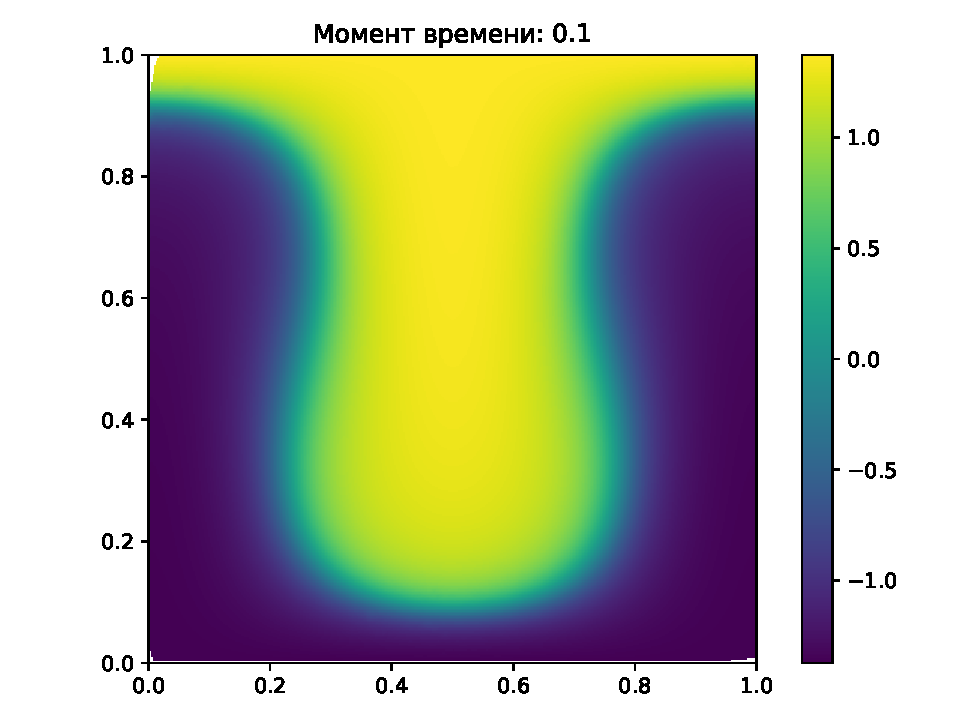
\includegraphics[width=8cm]{pictures/p5.pdf}
    \end{figure}
    \begin{figure}[H]
        \centering
        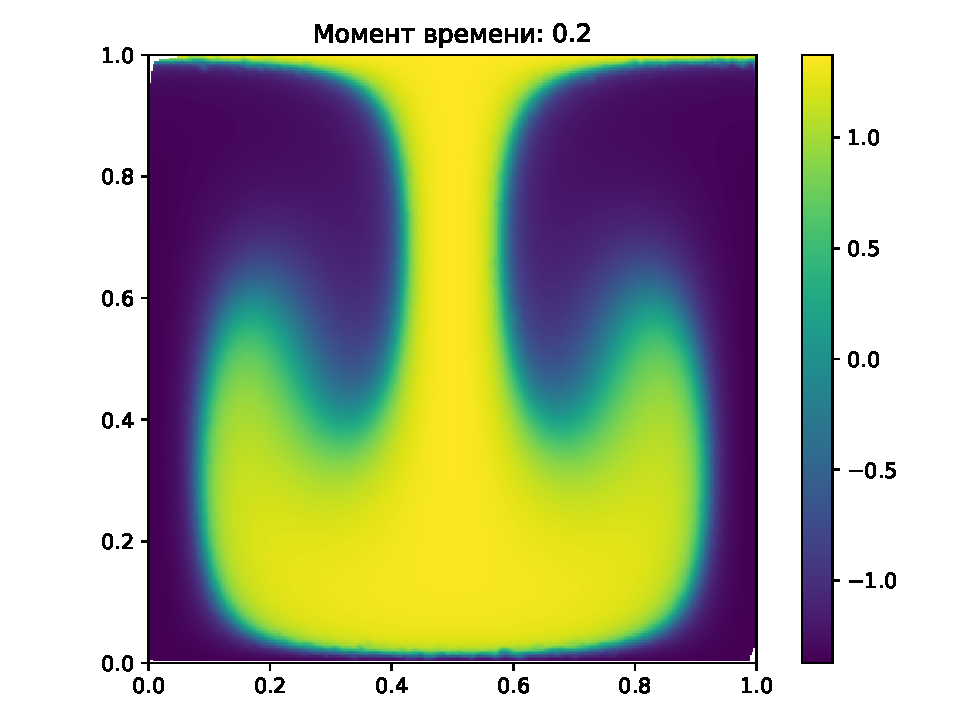
\includegraphics[width=8cm]{pictures/p10.pdf}
        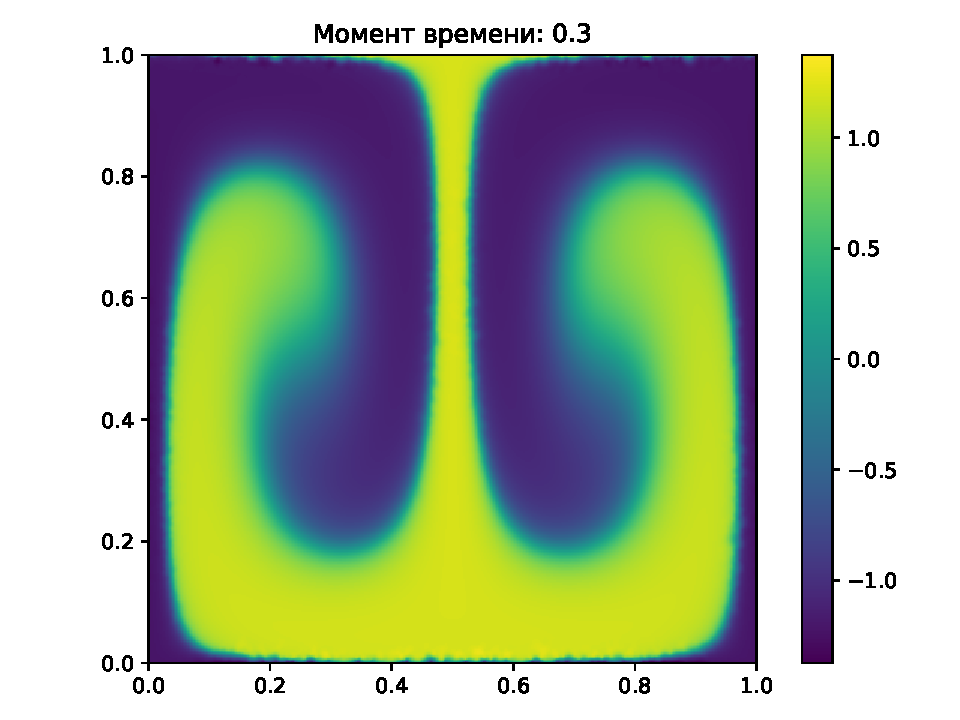
\includegraphics[width=8cm]{pictures/p15.pdf}
    \end{figure}
    \begin{figure}[H]
        \centering
        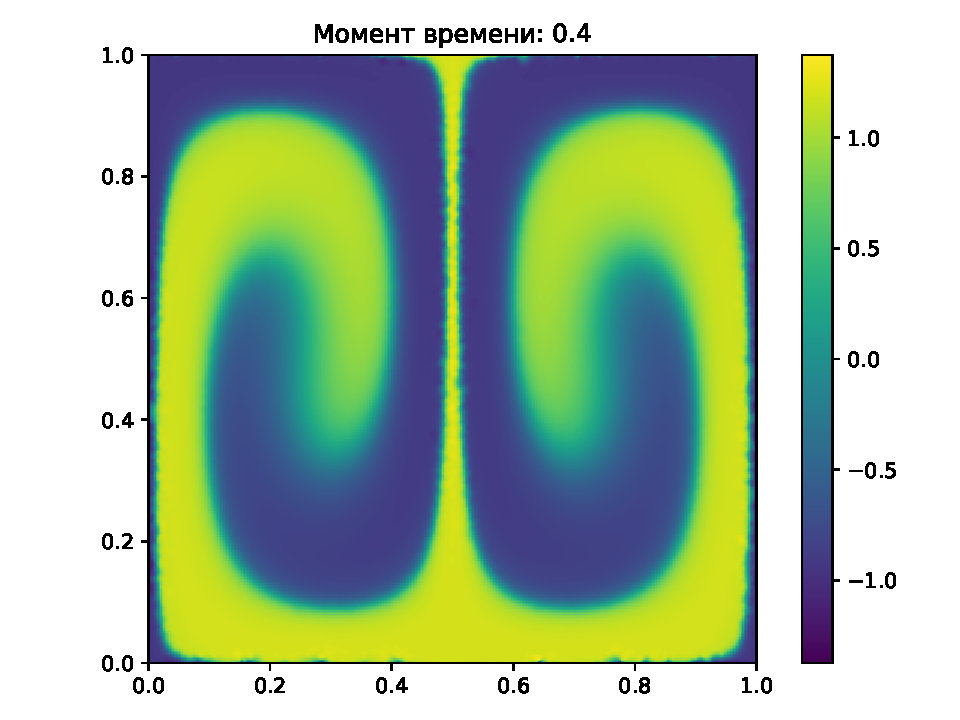
\includegraphics[width=8cm]{pictures/p20.pdf}
    \end{figure}

        